% !TeX root = repressed-anger.tex

\section{Classification Techniques}
\label{ch:algorithms}

The aim of this section has two purposes. The first one, is to make an introduction of the basic concepts of classification, which is essential for the detection of repressed anger. The second one, is to explain how the algorithms used in this study work.

\subsection{Fundamentals of Classification}

According to \cite{voznika2007data}, classification can be defined as the task of predicting an outcome from a given input. This outcome is produced by the process of mapping a group of characteristics present in the input to a certain category. In other words, it consists in assigning objects (the input) to one of several predefined classes (the outcome) \cite{pang2006introduction}. Examples of classification can be found in everyday life, such as e-mail spam detection, news classifiers, \acrfull{ocr}, animal kingdom classification (see Figure \ref{fig:animal_classification}), among many others.

\begin{figure}[!htp]
  \center
  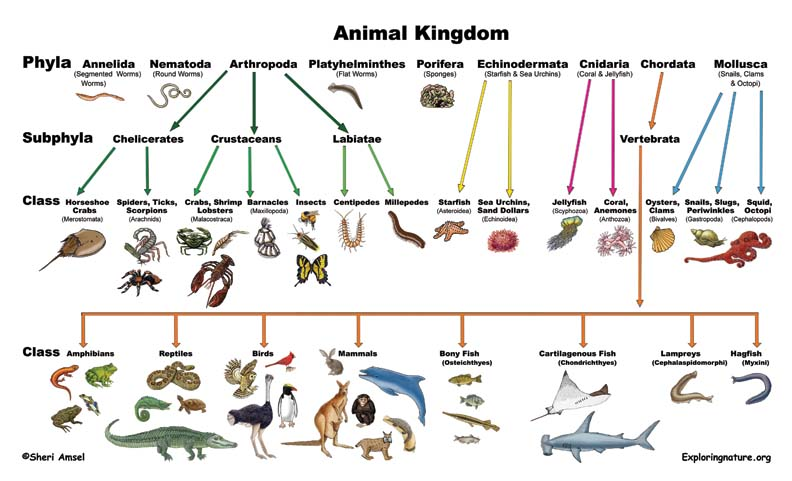
\includegraphics[width=0.7\textwidth]{figures/animal_classification}
  \caption{Classification of animals. The image is extracted from Exploring Nature.}
  \label{fig:animal_classification}
\end{figure}

The input data for a classification task is composed by a collection of records, the dataset. In the same time, each record, also known as an instance, is composed by a set attributes. From all these attributes there is one considered special, which is called the target attribute or the class label. Regular attributes can be both discrete or continuous values. For the values signed for the class label, however, they must be discrete. This characteristic is what distinguishes classification form regression. Table \ref{tab:clasiffication_table} shows a sample dataset for animal classification into the following categories: amphibian, bird, fish or mammal.

\begin{table}[!htp]
\centering
\begin{tabular}{ |c|c|c|c|c|c|c|c| }
\hline
Common Name & Hair & Feathers & Eggs & Milk & Aquatic & Legs & Class Label \\ \hline
antelope & Yes & No & No & No & No & 4 & mammal \\ \hline
catfish & No & No & Yes & No & Yes & 0 & fish \\ \hline
dolphin & No & No & No & Yes & Yes & 0 & mammal \\ \hline
dove & No & Yes & Yes & No & No & 2 & bird \\ \hline
duck & No & Yes & Yes & No & Yes & 2 & bird \\ \hline
elephant & Yes & Yes & No & Yes & No & 4 & mammal \\ \hline
flamingo & Yes & Yes & Yes & No & No & 2 & bird \\ \hline
frog & No & No & Yes & No & Yes & 4 & amphibian \\ \hline
fruit bat & Yes & No & No & Yes & No & 2 & mammal \\ \hline
gull & No & Yes & Yes & No & Yes & 2 & bird \\ \hline
herring & No & No & Yes & No & Yes & 0 & fish \\ \hline
kiwi & No & No & Yes & No & No & 2 & bird \\ \hline
lark & No & Yes & Yes & No & No & 2 & bird \\ \hline
lynx & Yes & No & No & Yes & No & 4 & mammal \\ \hline
mole & Yes & No & No & Yes & No & 4 & mammal \\ \hline
mongoose & Yes & No & No & Yes & No & 4 & mammal \\ \hline
newt & No & No & Yes & No & Yes & 4 & amphibian \\
\hline
\end{tabular}
\caption{Animal kingdom dataset.}
\label{tab:clasiffication_table}
\end{table}

Tan Pang-Ning et al. propose a more mathematical definition of classification stating that it is the process of learning a target function $f$, also known as classification model, that maps each attribute set $x$ to one of the predefined class labels $y$.

\begin{figure}[!htp]
  \center
  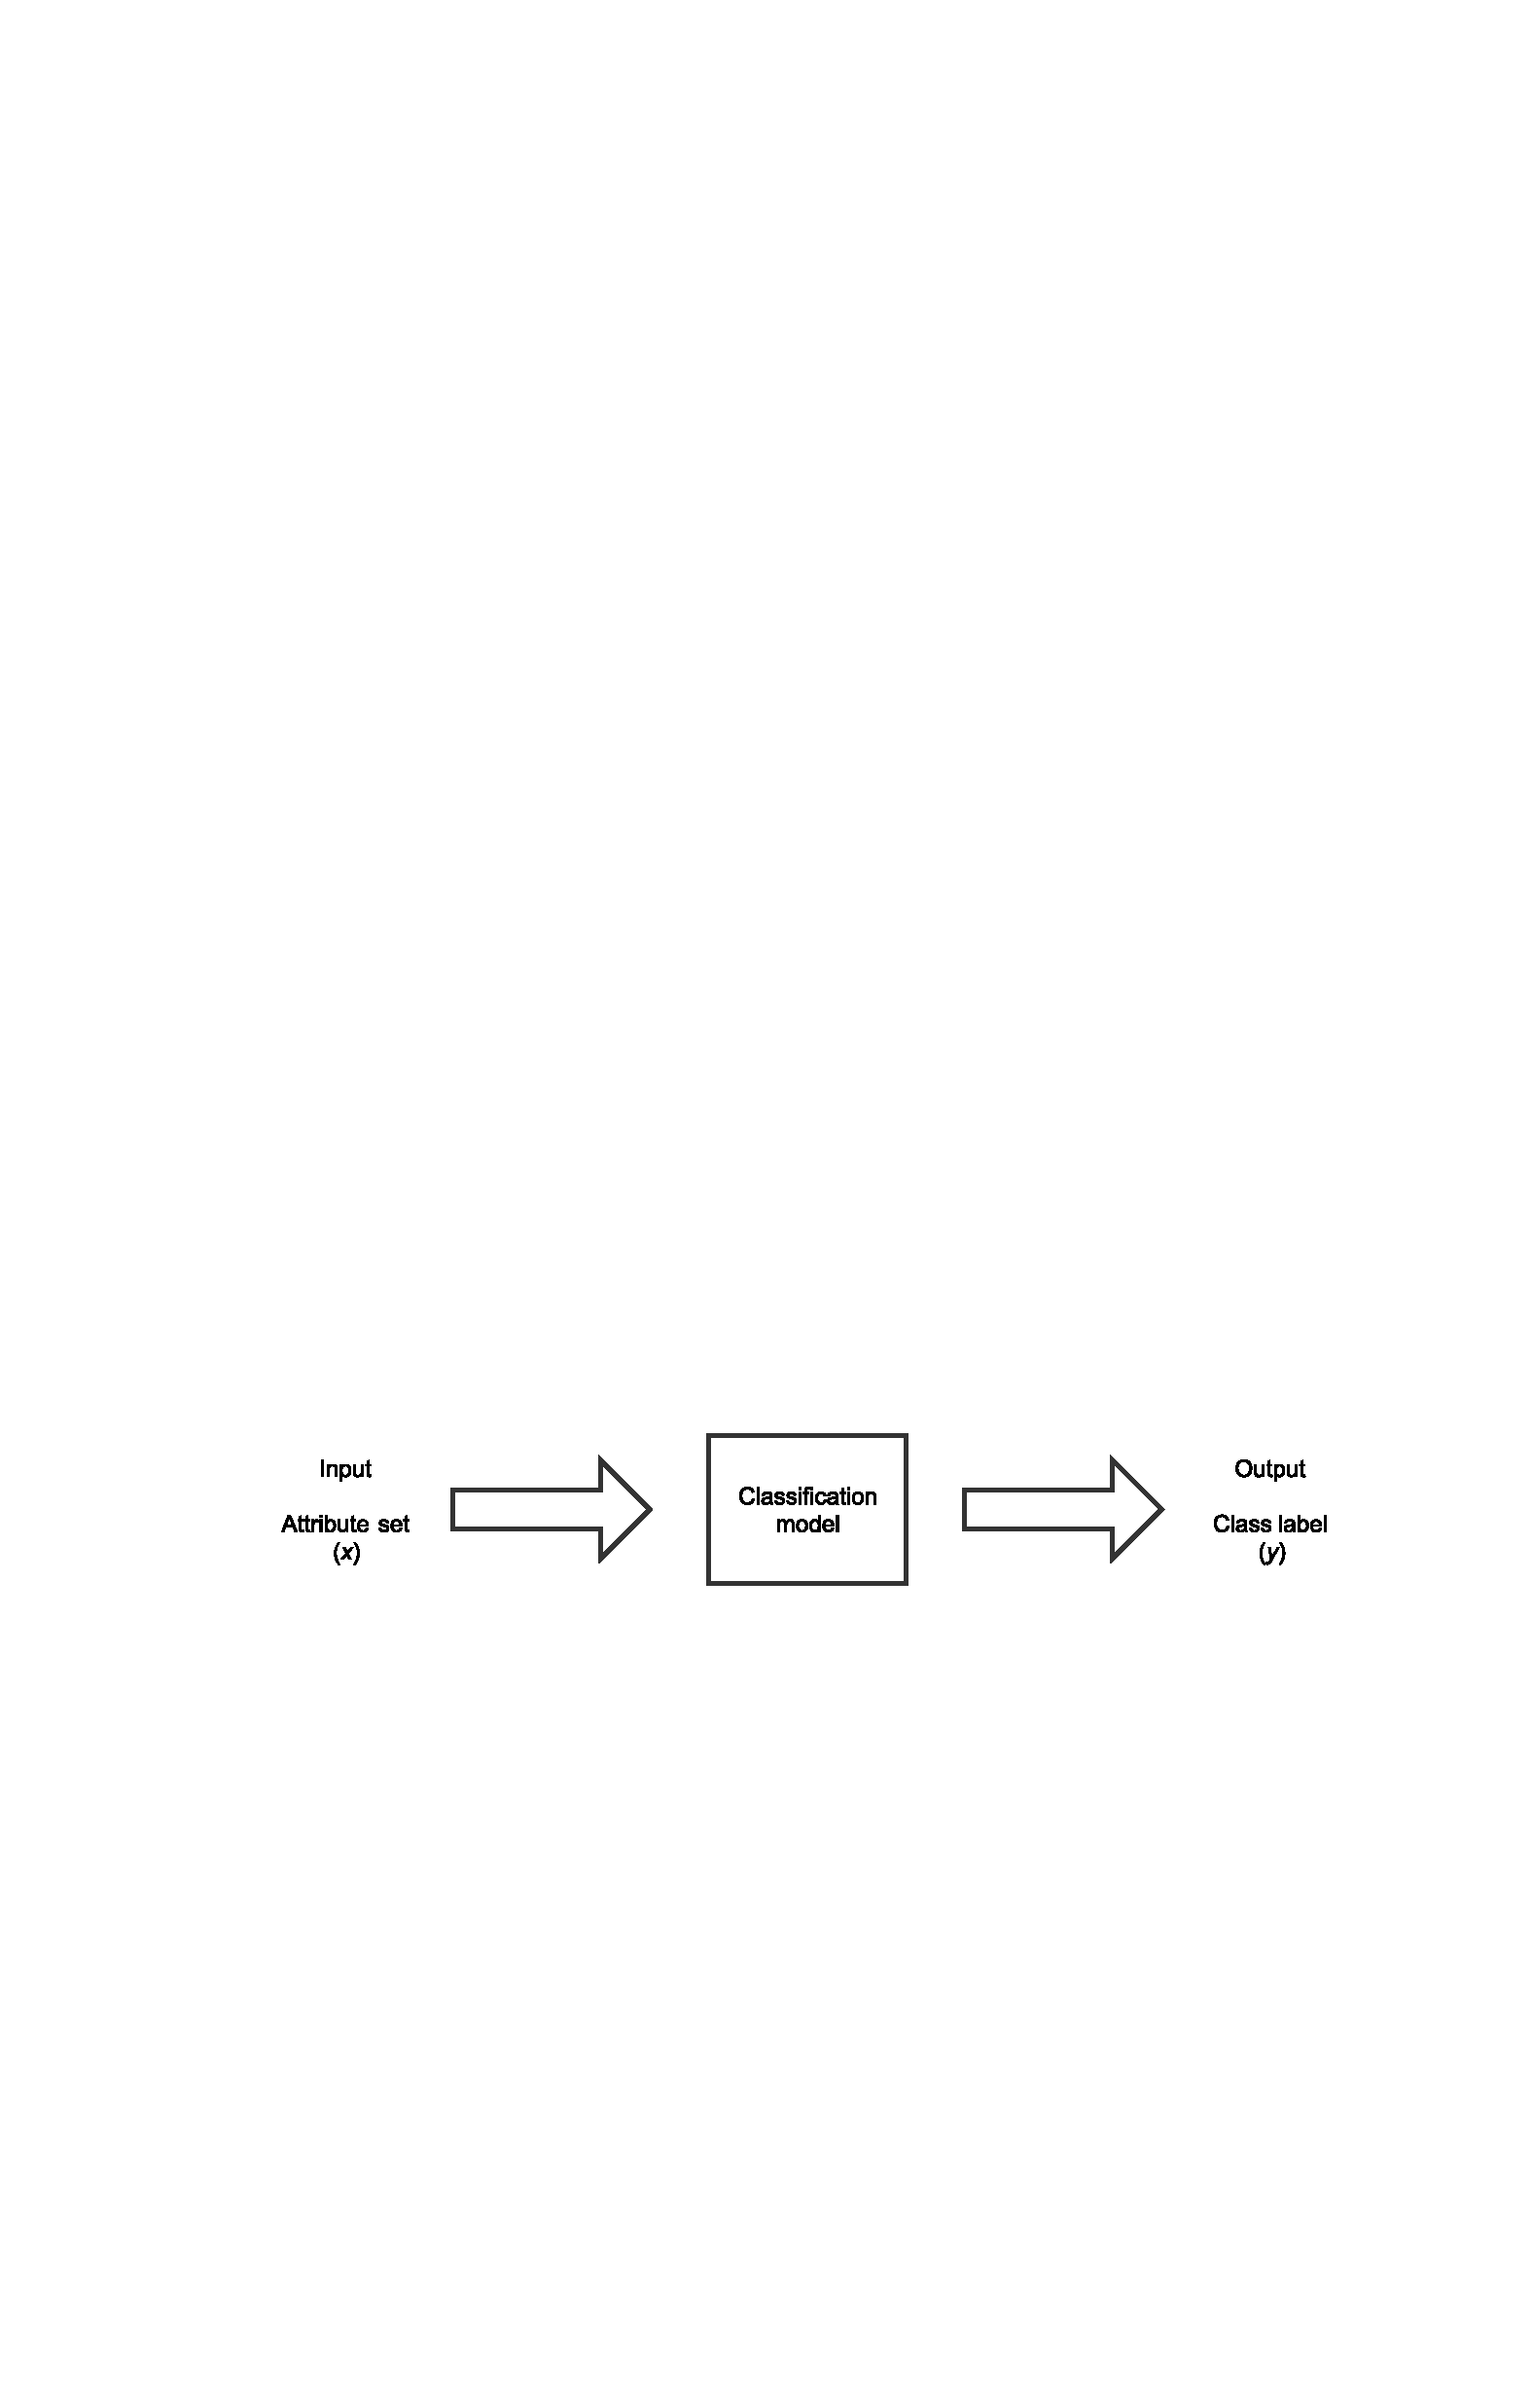
\includegraphics[width=\textwidth]{figures/classification}
  \caption{Classification as a task of mapping a set attributes $x$ into its fitting class label $y$.}
  \label{fig:classification_task}
\end{figure}

A classification model is useful for the following purposes \cite{pang2006introduction}:

\begin{itemize}
\item \textbf{Descriptive Modeling:} Since a classification model presents the main features of the data, it can serve as an explanatory tool to distinguish between instances of different categories \cite{madigan2002descriptive}.

\item \textbf{Predictive Modeling:} A classification model can also be used to predict the class label of an unknown new instance. As shown in Figure \ref{fig:classification_task}, a classification model can be represented as a black box that automatically assigns a class label to an instance by providing its attribute set.
\end{itemize}

It is important to remark that classification techniques perform their best when used for predicting or describing datasets which its class label is binary or nominal, Since they no consider properties such ordinality or the implicit order among the categories, they become ineffective with ordinal class labels \cite{frank2001simple}.

\subsection{General classification problem solving}

For general classification problems solving, popular techniques consists on a process that starts with building classification models from a sample dataset \cite{witten2005data}. Each technique depends on a learning algorithm witch is in charge of generating the classification model. A good model should define the relationship between the input attribute set and its belonging category that suits the best. Therefore the model should be valid for both, the sample data used to generate the model and also for new unknown instances. Among popular classification techniques \acrfull{svm}, \acrfullpl{nn}, Naive Bayes or \acrfullpl{dt} can be found \cite{garje2016sentiment}.

\begin{figure}[!htp]
  \center
  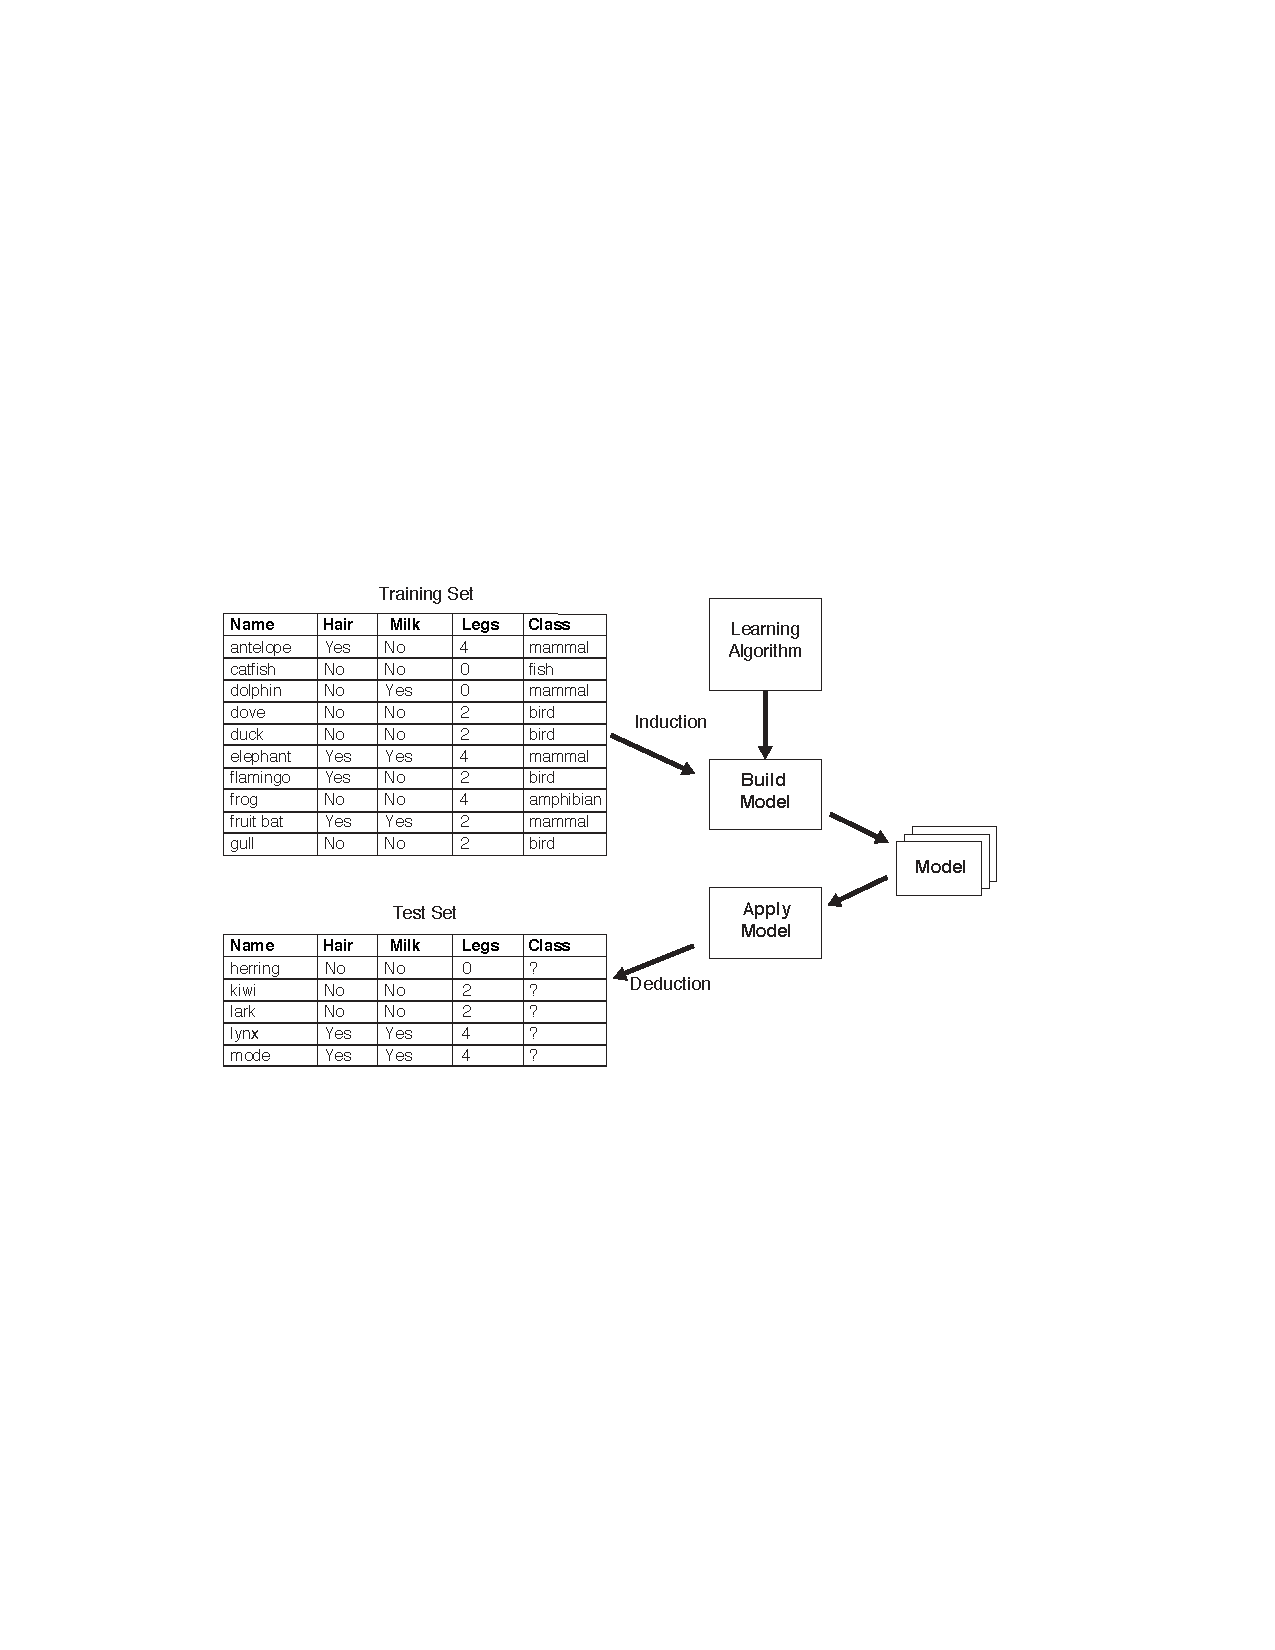
\includegraphics[width=0.7\textwidth]{figures/classification_problem_solving}
  \caption{General approach for classification model building and new instance category prediction.}
  \label{fig:classification_problem}
\end{figure}

As shown in the Figure \ref{fig:classification_problem}, to solve a classification problem a sample dataset must be provided as a training set. This sample is used to build the classification model according to the learning algorithm. After the model is built, it is applied to unlabeled dataset, also called the test set, to predict the categories of each instances of the records. To measure how good the model is, there is only need to count the number of instances have been correctly and incorrectly classified from the test set. Usually, to represent system's performance values, a confusion matrix is used \cite{hamilton2000confusion}. 


\begin{table}[!htp]
\centering
\begin{tabular}{ |c|c|c|c| }
\hline
\multicolumn{2}{|c|}{} & \multicolumn{2}{c|}{Predicted Class} \\
\hhline{~~--}
\multicolumn{2}{|c|}{} & $Class = Yes$ & $Class = No$ \\ \hline
\multirow{2}{*}{Actual Class} & $Class = Yes$ & a & b \\
\hhline{~---}
& $Class = No$ & c & d \\
\hline
\end{tabular}
\caption{Confusion matrix of a binary classification.}
\label{tab:confusion_matrix}
\end{table}

As a example, Table \ref{tab:confusion_matrix} represents the confusion matrix of a binary classification problem. 
\iffalse
There are two possible classes for an instance to be assigned, $Yes$ and $No$

[STARTS COPY PASTE]

Evaluation of the performance of a classification model is based on the counts of test records correctly and incorrectly predicted by the model. These counts are tabulated in a table known as a confusion matrix. Table 4.2 depicts the confusion matrix for a binary classification problem. Each entry fij in this table denotes the number of records from class i predicted to be of class j. For instance, f01 is the number of records from class 0 incorrectly predicted as class 1. Based on the entries in the confusion matrix, the total number of correct predictions made by the model is (f11 + f00) and the total number of incorrect predictions is (f10 + f01).
Although a confusion matrix provides the information needed to determine how well a classification model performs, summarizing this information with a single number would make it more convenient to compare the performance of different models. This can be done using a performance metric such as accuracy, which is defined as follows:

Accuracy = Number of correct predictions = f11 + f00 . (4.1) Total number of predictions f11 + f10 + f01 + f00

Equivalently, the performance of a model can be expressed in terms of its error rate, which is given by the following equation:

Error rate = Number of wrong predictions = f10 + f01 . (4.2) Total number of predictions f11 + f10 + f01 + f00

Most classification algorithms seek models that attain the highest accuracy, or equivalently, the lowest error rate when applied to the test set. We will revisit the topic of model evaluation in subsection 4.5.

\subsection{Support Vector Machine}

There are four main advantages: Firstly it has a regularisation parameter, which makes the user think about avoiding over-fitting. Secondly it uses the kernel trick, so you can build in expert knowledge about the problem via engineering the kernel. Thirdly an SVM is defined by a convex optimisation problem (no local minima) for which there are efficient methods (e.g. SMO). Lastly, it is an approximation to a bound on the test error rate, and there is a substantial body of theory behind it which suggests it should be a good idea.
The disadvantages are that the theory only really covers the determination of the parameters for a given value of the regularisation and kernel parameters and choice of kernel. In a way the SVM moves the problem of over-fitting from optimising the parameters to model selection. Sadly kernel models can be quite sensitive to over-fitting the model selection criterion \cite{cawley2010over}

--------------------

SVMs are a new promising non-linear, non-parametric classification tech- nique, which already showed good results in the medical diagnostics, optical character recognition, elec- tric load forecasting and other fields.

Suitable for binary classification tasks.

The advantages of the SVM technique can be summarised as follows \cite{auria2008support}:

\begin{enumerate}
\item By introducing the kernel, SVMs gain flexibility in the choice of the form of the threshold separating solvent from insolvent companies, which needs not be linear and even needs not have the same func- tional form for all data, since its function is non-parametric and operates locally. As a consequence they can work with financial ratios, which show a non-monotone relation to the score and to the probability of default, or which are non-linearly dependent, and this without needing any specific work on each non-monotone variable.
\item Since the kernel implicitly contains a non-linear transformation, no assumptions about the functional form of the transformation, which makes data linearly separable, is necessary. The transformation oc- curs implicitly on a robust theoretical basis and human expertise judgement beforehand is not needed.
\item SVMs provide a good out-of-sample generalization, if the parameters C and r (in the case of a Gaussian kernel) are appropriately chosen. This means that, by choosing an appropriate generalization grade, SVMs can be robust, even when the training sample has some bias
\item SVMs deliver a unique solution, since the optimality problem is convex. This is an advantage compared to Neural Networks, which have multiple solutions associated with local minima and for this reason may not be robust over different samples.
\item With the choice of an appropriate kernel, such as the Gaussian kernel, one can put more stress on the similarity between companies, because the more similar the financial structure of two companies is, the higher is the value of the kernel. Thus when classifying a new company, the values of its financial ratios are compared with the ones of the support vectors of the training sample which are more similar to this new company. This company is then classified according to with which group it has the greatest similarity.
\end{enumerate}

--------------------------

Furthermore, $K(\bm{x}i, \bm{x}j ) \equiv \phi(\bm{x}_i)^T \phi(\bm{x}_j)$ is called the kernel function.

four basic kernels \cite{hsu2003practical}:

\begin{itemize}
\item \textbf{Linear:} $K(\bm{x}_i,\bm{x}_j) = \bm{x}^T_i \bm{x}_j$.
\item \textbf{Polynomial:} $K(\bm{x}_i,\bm{x}_j) = (\gamma \bm{x}^T_i \bm{x}_j + r)^d, \gamma > 0$.
\item \textbf{Radial Basis Function (RBF):} $K(\bm{x}_i,\bm{x}_j) = \exp(−\gamma \lVert \bm{x}_i − \bm{x}_j \rVert ^2),\gamma > 0$.
\item \textbf{Sigmoid:} $K(\bm{x}_i,\bm{x}_j) = \tanh(\gamma \bm{x}^T_i\bm{x}_j + r)$.
\end{itemize}

Here, $\gamma$, $r$, and $d$ are kernel parameters.

--------------------------

Support vector machines (SVM) were originally designed for binary classification \cite{hsu2002comparison}.

solving multi-class SVM in one step: “all-together” methods: [25], [27] and [7]. We then compare their performance with three methods based on binary classifications: “one-against-all,” “one-against-one,” and DAGSVM [23]. Our experiments indicate that the “one-against-one” and DAG methods are more suitable for practical use than the other methods. 

--------------------------

asdasdasd \cite{berwick2003idiot}

\begin{figure}[!htp]
  \center
  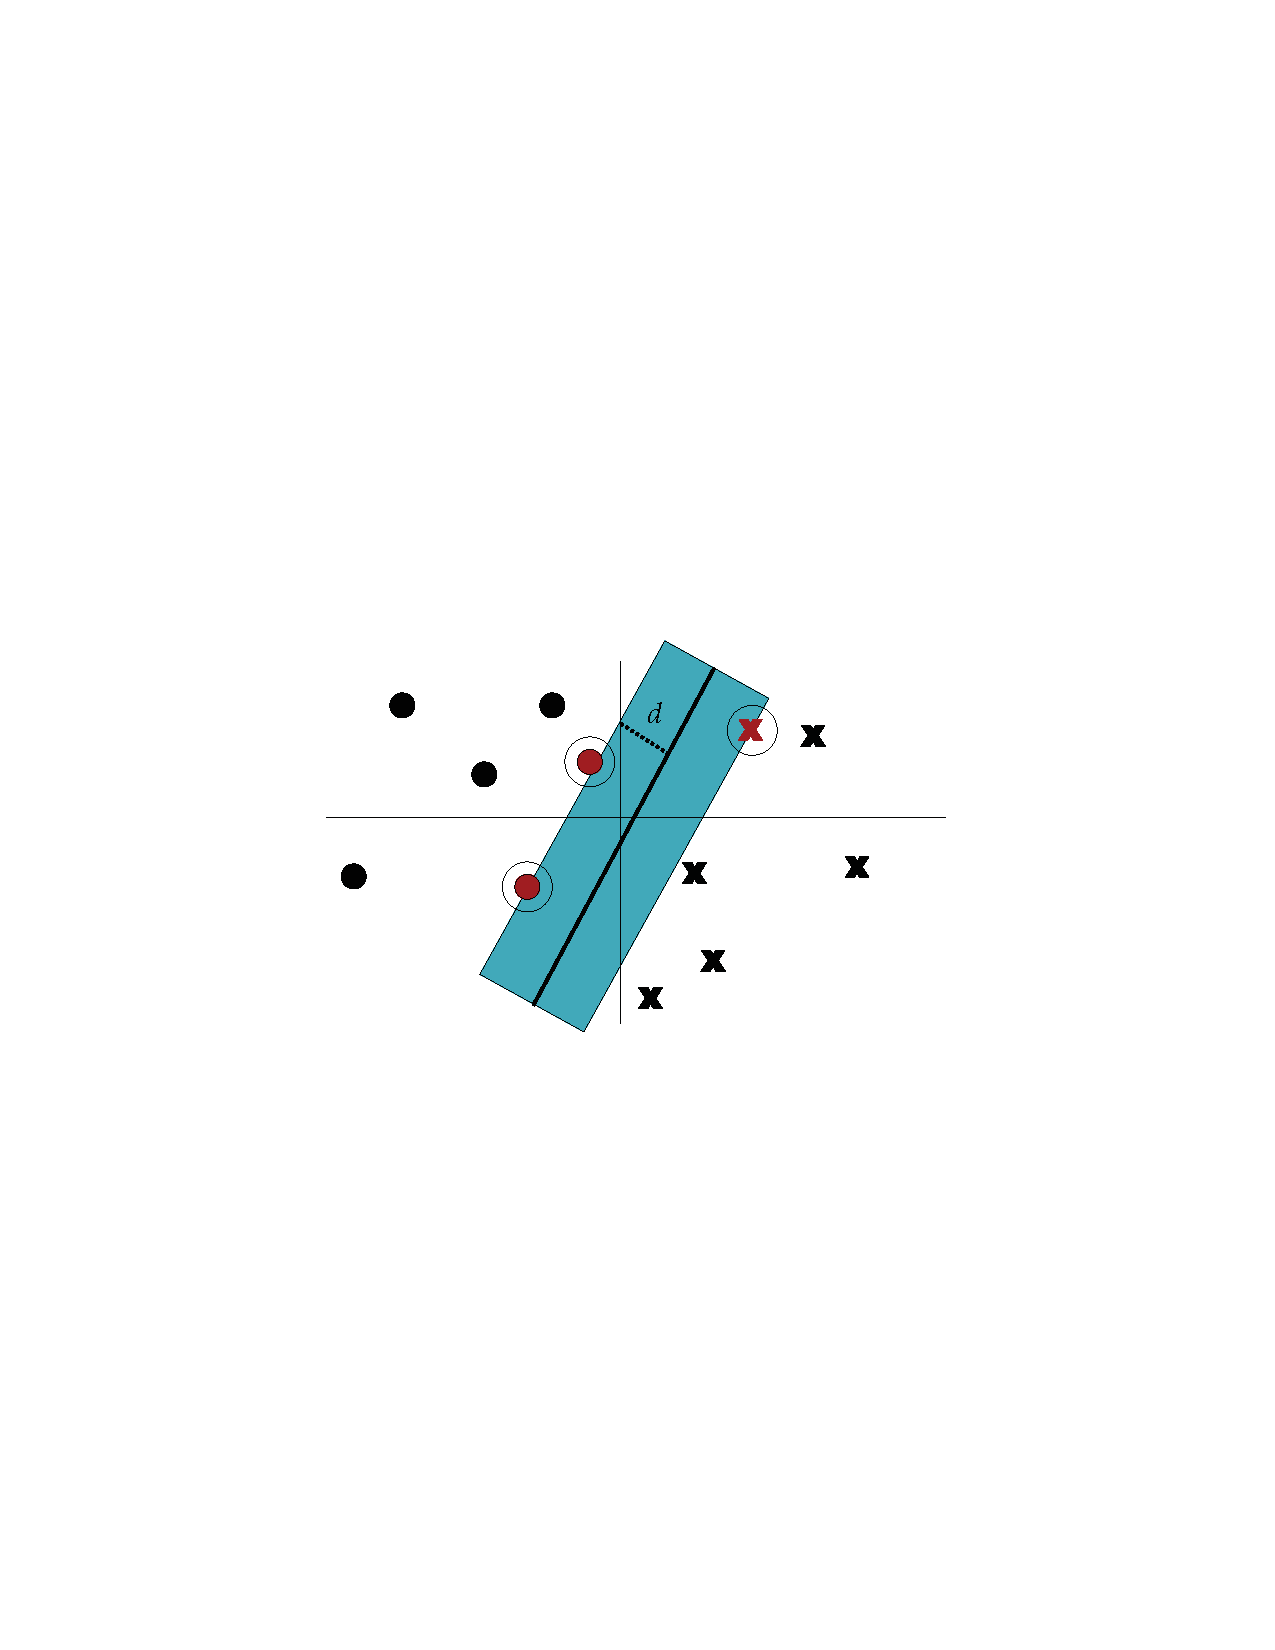
\includegraphics[width=0.6\textwidth]{figures/hyperplane}
  \caption{hyperplane}
  \label{fig:hyperplane}
\end{figure}

\subsection{K-Nearest Neighbor}

\subsection{Neural Networks}

\fi